\section{问题重述与分析}
\subsection{问题背景与研究任务}
热风烘干通过外部空气向药材供热，并将药材内部迁移至表面的水分带走。表面先接触热风，内部升温与失水存在滞后；随着含水率降低，导热能力、储热能力和水分扩散能力也会变化。因此，外部空气接近恒温，并不表示药材已经干燥，更不能仅凭表面含水率判断整个药材是否达标。题目给出的初始药材近似为长25 cm、半径2 cm的圆柱，初始温度为28 $^\circ$C，初始干基含水率为2.55 kg/kg，烘房初期温度及水分变量见附件1，烘干过程的半径变化见附件2。

问题一要求采用附录2的参数，求出前1800 s的温度场和含水率场，并按指定时间与径向位置给出结果。问题二改用附录3的经验物性，建立适用于整个过程的热质传递模型，输出前3 h的温湿分布。问题三在问题二的物性模型上，确定所有位置含水率均低于0.15 kg/kg的首次时刻，并给出全程水分分布。问题四进一步使用附件2的变化半径和附录4的经验公式，确定收缩药材的干燥时长。四问均需按附件模板输出完整Excel结果。

\subsection{模型选择与需要区分的量}
本文采用圆柱径向热质耦合模型，以局部温度和干基含水率为状态变量。选择空间分布模型的直接原因是题目同时规定中心、内部和表面的输出位置。一个平均温度或平均含水率的常微分方程无法恢复这些剖面，也不能直接满足“各处达标”的判据。对初始尺度，端面总面积与侧面积之比为$R_0/L=0.08$，说明侧向传递具有较大的交换面积，但这一面积比本身不是一维近似的误差上界。本文先建立径向主模型，再以轴对称二维计算检验端面作用。

问题四的关键是明确网格所代表的对象。半径随时间变小，可以描述材料整体收缩，也可以只表示在静止场上截取的计算区域缩小；两者的坐标公式相似，物理质量预算却不同。本文将$\xi=r/R(t)$规定为材料坐标，使同一$\xi$对应同一干固体材料点，并从干固体和水的连续方程推导含水率方程。一般的任意拉格朗日--欧拉描述需要区分材料速度与网格速度\cite{donea2004}，这里采用二者相等的特例。

另一个关键是数据覆盖范围。附件1只覆盖0至4 h，而达标时刻超过50 h。因此，4 h以后的空气边界不能被称为附件实测值。本文保留已有固定半径结果所采用的末点延续作为问题三的明确情景；问题四推荐采用末一小时观测均值平台，并同时计算末点平台和名义平台。两问的物性与平台不同，不能把它们的时间差全部归因于收缩。收缩作用另由同物性、同平台的配对计算估计。

\section{模型假设、符号与数据处理}
\subsection{模型假设及其适用范围}
假设药材在初始时具有轴对称、均匀的温度和含水率，热风在侧面形成空间均匀、随时间变化的边界。主模型忽略周向和轴向差异；关于轴向近似的适用程度，由第\ref{sec:endface}节的二维对照单独判断。问题一至三保持圆柱半径和长度不变，问题四保持长度不变，半径按附件2规定，并采用均匀的径向随体形变。附件只给出外轮廓半径，未给局部位移和孔隙信息，故均匀形变是模型闭合所用的假设，而不是从半径曲线唯一推得的事实。

假设干固体不发生反应和损失，以独立干固体密度$s$记录其质量。固定半径时$s$为空间和时间常量；均匀径向收缩时$s$在空间上均匀，随体积改变而变化。题目给出的$\rho(C)$、$c_p(C)$、$k(C)$及$D(C,T)$均按相应问题使用。尤其将$\rho(C)c_p(C)$解释为温度方程的经验有效体积热容，记作$a(C)$，不再额外强制$\rho(C)/(1+C)$等于守恒干固体密度。这个区分对收缩模型不可省略，其一致性检验见第\ref{sec:density}节。

假设水分相对于干固体的迁移可由有效扩散通量表示，表面采用题目系数构成的经验Robin传质边界。用$C_{\mathrm{eq}}$表示与空气状态对应的等效表面平衡含水变量，并取$C_{\mathrm{eq}}=C_{\mathrm{air}}$。由于附件没有吸附等温线和分配系数，这一关系属于有效经验映射；它不意味着空气与药材两种kg/kg变量具有同一个质量分母。

温度与含水率通过经验物性相互作用，不引入题目未给定的相变潜热、压力驱动和化学反应参数。因此，温度方程是给定资料下的有效导热近似，不是包含全部潜热与多相焓输运的能量守恒模型。本文不据此计算能耗，也不把数值收支误差小解释为真实工艺已经获得实验验证。

\subsection{主要符号与单位}
全文采用SI单位计算，制表时将时间转换为题目指定的秒或小时，将径向距离转换为厘米。温度场以$T$表示，单位为$^\circ$C；进入指数经验公式时使用绝对温度$\Theta=T+273.15$，单位为K。温差在两种温标下数值相同，但指数中的温度不能直接使用摄氏数值。

\begin{description}[style=nextline,leftmargin=3.8em,labelwidth=3.2em]
  \item[$r,\xi$] $r$为距圆柱轴线的径向距离，单位m；$\xi=r/R(t)\in[0,1]$为归一化径向坐标。固定半径模型中也使用此网格记法。
  \item[$R,L$] $R(t)$为当前半径，$R_0=0.02$ m；$L=0.25$ m为固定长度。二维对照使用轴向半长度$H=L/2$。
  \item[$C$] 干基含水率，定义为水质量与干固体质量之比，单位kg水/kg干固体。$C_s$为侧表面值，$C_{\max}$为计算域内最大值。
  \item[$s,v,w$] $s$为单位当前体积内的干固体质量，单位kg/m$^3$；$v$为干固体径向速度，$w$为网格径向速度，单位m/s。
  \item[$a,k,D$] $a=\rho_{\mathrm{eff}}c_p$为有效体积热容，单位J/(m$^3$\,K)；$k$为导热系数，单位W/(m\,K)；$D$为水分有效扩散系数，单位m$^2$/s。
  \item[$h_T,h_m$] $h_T=25$ W/(m$^2$\,K)为换热系数；$h_m=8\times10^{-7}$ m/s为经验传质系数。三套物性模型均使用这两个系数。
  \item[$t_*,\overline C$] $t_*$为全域最大含水率首次跨过阈值的时间；$\overline C=M_w/M_d$为以总干质量归一化的平均含水率。
\end{description}

\subsection{观测区间内的插值}
附件1包含241个观测时刻，间隔为60 s，范围为0至14400 s；附件2包含145个半径观测值，间隔为1800 s，范围为0至259200 s。两份数据均保留原始采样值，不为了获得光滑图像而平滑或改写平台波动。求解时，对温度、空气水分变量和半径分别使用分段三次Hermite保形插值（PCHIP）。这一类局部插值通过邻近割线确定节点斜率，使分段单调数据在区间内保持单调\cite{fritsch1984}，适合处理升温段与接近平稳的平台段。其作用是构造观测点之间的连续输入，不是增加观测信息。

图\ref{fig:boundary}显示温度在初期持续升高，后段接近50 $^\circ$C；空气水分变量则逐渐接近0.05。采用线性插值的替代计算用于检查插值选择对问题四达标时间的影响，结果在第\ref{sec:convergence}节给出。本文将采样分辨率、积分时间步长和结果输出间隔分别处理：60 s采样并不限制数值时间步长只能取60 s，1 s输出也不意味着计算误差为1 s。

\begin{figure}[htbp]
\centering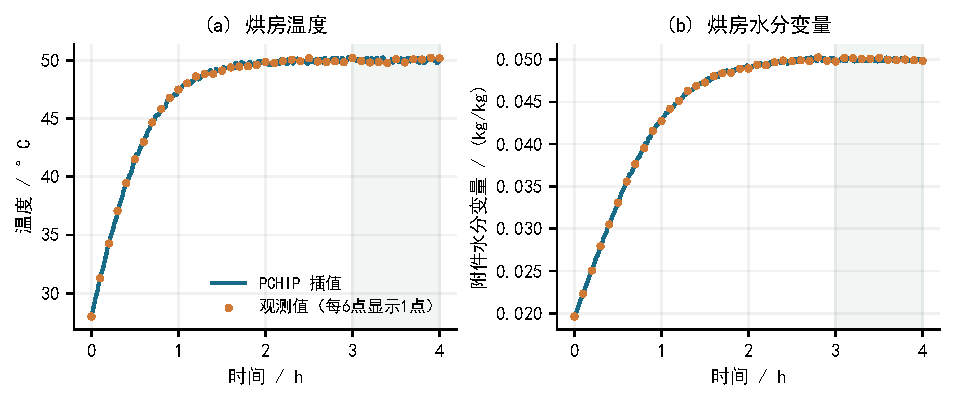
\includegraphics[width=\textwidth]{figures/boundary.pdf}
\caption{附件1的烘房观测与区间内插值。浅色区域为用于计算平台均值的3至4 h；图中散点为原始观测的等间隔显示子集。}\label{fig:boundary}
\end{figure}

图\ref{fig:radius}给出附件2的半径曲线及其在归一化方程中的几何倍率。半径在前12 h由2 cm减至1.248 cm，之后变化明显放缓；36 h至问题四终点的记录约为1.200 cm。主结果的51.09 h位于半径实测区间内，因而计算不需要把半径外推到72 h以后。图中几何倍率仅表示在同一物性值下，归一化扩散和表面交换系数随尺度的变化，不能独立代替非线性过程的求解。

\begin{figure}[htbp]
\centering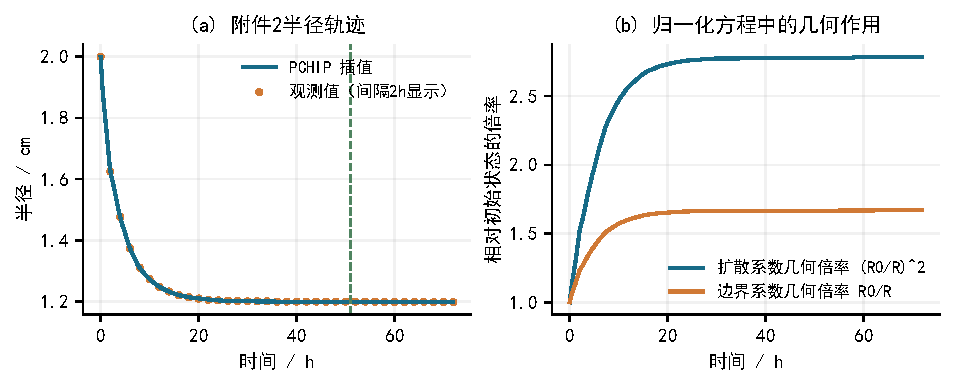
\includegraphics[width=\textwidth]{figures/radius.pdf}
\caption{规定半径及其几何作用。左图虚线标记问题四达标时刻；右图中的倍率相对于初始半径计算。}\label{fig:radius}
\end{figure}

\subsection{4 h以后的边界延续}
末一小时包含3 h和4 h两个端点，共61个观测值。由于采样间隔相等，本文以这些值的算术平均构造恒定平台：
\begin{equation}
 T_{\mathrm{air},\mathrm{mean}}=49.9989344262\ ^\circ\mathrm C,
 \qquad C_{\mathrm{eq},\mathrm{mean}}=0.049987540984.
 \label{eq:mean-boundary}
\end{equation}
这一平台使用了后段全部采样信息，降低了单个末点波动对长期延续的影响。它与名义的50 $^\circ$C、0.05平台接近，因而作为问题四的推荐情景。另一方面，附件未明确规定4 h后的工艺控制，此推荐仍然是一项延续假设，不能称作已知边界条件。

另外保留两种情景：末点保持为50.165 $^\circ$C和0.04986；名义平台为50 $^\circ$C和0.05。所有情景在0至4 h完全使用同一插值，只有$t>4$ h时采用各自的恒定值。问题三主结果使用末点保持；问题四主结果使用式\eqref{eq:mean-boundary}。均值平台在4 h右侧可能相对末次采样产生一个小跳变，数值计算按分段定义直接处理，没有虚构一段过渡观测。

\section{固定圆柱热质传递模型与数值方法}
\subsection{控制方程及初边值条件}
在半径固定的圆柱内，温度与水分的径向模型为
\begin{align}
 a(C)\frac{\partial T}{\partial t}
 &=\frac1r\frac{\partial}{\partial r}
   \left(rk(C)\frac{\partial T}{\partial r}\right),\label{eq:fixed-heat}\\
 \frac{\partial C}{\partial t}
 &=\frac1r\frac{\partial}{\partial r}
   \left(rD(C,\Theta)\frac{\partial C}{\partial r}\right).
 \label{eq:fixed-moisture}
\end{align}
式\eqref{eq:fixed-moisture}对应独立、均匀且不变的干固体密度。若写成真实水质量方程，其储存项与扩散通量均乘以$s$，因$s$为空间常量而可约去。由此得到的体积加权含水率也等于干质量加权含水率。这里的质量解释不依赖热学有效密度的数值变化。

轴线处的对称条件和侧面的交换条件为
\begin{align}
 T_r(0,t)&=0, & C_r(0,t)&=0,\label{eq:center}\\
 -kT_r(R_0,t)&=h_T(T_s-T_{\mathrm{air}}), &
 -DC_r(R_0,t)&=h_m(C_s-C_{\mathrm{eq}}).
 \label{eq:robin}
\end{align}
这里将朝圆柱外的通量定义为正。预热时常有$T_s<T_{\mathrm{air}}$，故热通量为负，表示热量流入药材；干燥时$C_s>C_{\mathrm{eq}}$，水分通量为正，表示水向外迁移。这一符号约定同时用于边界离散与整体收支，避免将升温方向或排水方向写反。初始条件为
\begin{equation}
 T(r,0)=28\ ^\circ\mathrm C,\qquad C(r,0)=2.55,
 \qquad 0\le r\le R_0.\label{eq:initial}
\end{equation}

注意$D$、$k$均放在散度内部。含水率不均匀时，它们在空间中变化，因此不能将$\partial_r(rD C_r)/r$直接替换为$D(C_{rr}+C_r/r)$而遗漏系数梯度。有效体积热容乘以局部温度变化率；本文没有将其改写为$\partial_t(aT)$，后者会额外引入$a_tT$项，属于另一种热学闭合。

\subsection{三套经验物性的一致使用}
问题一仅采用附录2：
\begin{equation}
 a=820\times2600,\quad k=0.36,\quad
 D_1(C)=7\times10^{-9}\exp\left(-\frac{0.89}{C}\right).
 \label{eq:prop1}
\end{equation}
问题二和问题三从初始时刻起统一采用附录3，而不是在预热结束后才切换：
\begin{align}
 \rho_{\mathrm{eff},23}&=650+128C,&
 c_{p,23}&=1450+2736\frac{C}{C+1},\notag\\
 k_{23}&=0.21+0.38\frac{C}{C+1},&
 D_{23}&=2.4\times10^{-3}
 \exp\left(-\frac{0.45}{C}-\frac{3850}{\Theta}\right).
 \label{eq:prop23}
\end{align}
问题四使用附录4：
\begin{align}
 \rho_{\mathrm{eff},4}&=760+90C,&
 c_{p,4}&=1850+2150\frac{C}{C+1},\notag\\
 k_4&=0.12+0.20\frac{C}{C+1},&
 D_4&=4.2\times10^{-4}
 \exp\left(-\frac{0.30}{C}-\frac{3850}{\Theta}\right).
 \label{eq:prop4}
\end{align}
上述密度、比热容、导热系数和扩散系数的单位依次为kg/m$^3$、J/(kg\,K)、W/(m\,K)和m$^2$/s，$a_q=\rho_{\mathrm{eff},q}c_{p,q}$。物性表达式只按题号选择，不能用问题一的常数热物性去生成问题二的前半小时结果，也不能将问题三的参数和问题四的收缩混合后称为题目指定的第四问模型。

这些公式使系统具有双向的参数耦合：温度进入$D$，影响含水率变化；含水率又进入有效体积热容和导热系数，影响升温。对于$D=A\exp(-b/C-3850/\Theta)$，直接求导有
\begin{equation}
 \frac{\partial\log D}{\partial C}=\frac b{C^2}>0,
 \qquad \frac{\partial\log D}{\partial\Theta}
 =\frac{3850}{\Theta^2}>0.\label{eq:derivatives}
\end{equation}
因此，在其他条件相同的情况下，升温提高扩散能力，而失水降低扩散能力。干燥后期两种作用不再对称：温度已经接近平台，但低含水率仍使扩散系数下降，形成后期的缓慢失水段。这也说明用初始扩散系数估计全程达标时间缺少依据。

\subsection{圆柱控制体及界面通量}
有限体积法从每个控制体的收支出发，将相邻单元间的同一通量以相反符号加入两侧，从而实现离散局部守恒\cite{eymard2000}。本文取$N$个节点$\xi_i=i/(N-1)$，$i=0,\ldots,N-1$，首末节点分别位于轴线与表面；相邻节点中点为内部控制面，边界控制面为0和1。记控制面为$\xi_{i\pm1/2}$，则径向权重为
\begin{equation}
 V_i=\frac{\xi_{i+1/2}^2-\xi_{i-1/2}^2}{2},
 \qquad \sum_iV_i=\frac12.\label{eq:weights}
\end{equation}
首节点仍具有有限的半控制体，离散时无需在$r=0$直接计算$1/r$。表面也保留半控制体，而不是把边界节点当作无容量的代数节点。这样既避免轴线奇点，又能用同一组权重进行全局水分预算。

设$U$代表温度或含水率，$p$代表相应的导热或扩散系数。内部相邻节点的传递系数为
\begin{equation}
 G_{i+1/2}=\frac{\xi_{i+1/2}}{\Delta\xi}\,p_{i+1/2},
 \qquad \Delta\xi=\frac1{N-1}.\label{eq:conductance}
\end{equation}
热传导使用正的调和界面均值$k_{i+1/2}=2k_ik_{i+1}/(k_i+k_{i+1})$。水分扩散对低含水率十分敏感，直接平均两个端点的$D$可能不足以解析表面的干燥薄层。本文在线性重构的状态路径上计算
\begin{equation}
 D_{i+1/2}=\int_0^1D\bigl((1-\eta)C_i+\eta C_{i+1},
 (1-\eta)\Theta_i+\eta\Theta_{i+1}\bigr)\,\mathrm d\eta,
 \label{eq:edge-integral}
\end{equation}
并用8点Gauss--Legendre正权重求积实现。恒温时，式\eqref{eq:edge-integral}等价于Kirchhoff势对$C$的差商；温度同时变化时，它是沿重构状态路径的有效界面系数，本文不将其称作完整非线性边值问题的精确通量。该系数保持正值，因而不会因指数非线性引入负的数值扩散。独立自适应求积与此8点规则的比较见第\ref{sec:validation}节。

\subsection{隐式迭代与守恒预算}
将热方程容量记为$b_i=a_i$、水分方程容量记为$b_i=1$。在固定半径或材料坐标形式下，后向Euler离散可统一写为
\begin{align}
 b_iR_n^2V_i\frac{U_i^n-U_i^{n-1}}{\Delta t}
 ={}&G_{i+1/2}(U_{i+1}^n-U_i^n)
   -G_{i-1/2}(U_i^n-U_{i-1}^n)\notag\\
 &-\boldsymbol1_{i=N-1}R_nh(U_i^n-U_\infty^n),
 \label{eq:be-fvm}
\end{align}
轴线和表面之外的内部面项均取零；$R_n$为当前步半径，固定模型中始终为$R_0$。这里$h$分别为$h_T$和$h_m$。在随体模型中，$R_n^2$同时乘在新旧状态差上；不能只在新时刻乘$R_n^2$而将旧时刻改用$R_{n-1}^2$，否则将改变所离散的质量变量。

每个时间步以旧时刻状态作为迭代初值，按当前$T,C$更新容量与界面系数，分别解两个三对角线性系统，再用所得新场更新物性，直至
\begin{equation}
 \|T^{(m+1)}-T^{(m)}\|_\infty<10^{-7}\ ^\circ\mathrm C,
 \qquad \|C^{(m+1)}-C^{(m)}\|_\infty<10^{-9}.
 \label{eq:picard}
\end{equation}
三对角系统使用Thomas算法。对主结果，迭代不作欠松弛，四问各步实际最多迭代3次；程序还检查非有限值、非正含水率和迭代不收敛，不将这些情况作为可接受输出。每次线性求解的计算量随节点数线性增加，适合长时间的逐步推进。

主结果统一采用$N=81$、$\Delta t=0.5$ s、后向Euler。独立比较使用二阶后向差分BDF2，其时间导数为$(3U^n-4U^{n-1}+U^{n-2})/(2\Delta t)$，第一步以Euler启动。两者使用相同的空间通量和物性更新，从而把时间离散选择与模型结构选择分开。

对随体含水率方程，式\eqref{eq:be-fvm}在所有节点求和后，内部通量严格抵消，得到
\begin{equation}
 \sum_iV_i(C_i^n-C_i^{n-1})
 =-\Delta t\frac{h_m}{R_n}(C_s^n-C_{\mathrm{eq}}^n).
 \label{eq:discrete-budget}
\end{equation}
本文同时检查逐步与累计收支。该预算所守恒的是相对于固定干质量的含水量，热学有效密度没有出现在质量分母中。数值预算与网格收敛回答不同问题：前者检验离散通量和储存项是否一致，后者检验特定预测量对离散参数是否敏感；二者都不能单独验证材料运动假设。

\section{问题一：预热平衡阶段的温湿分布}
\subsection{参数设置与计算结果}
将式\eqref{eq:prop1}代入固定圆柱模型，采用附件1在0至1800 s的插值边界。该问题的温度方程为常系数，但水分扩散仍依赖局部含水率，所以不能把整个问题当作两个常系数扩散方程。计算结果按实际$r$位置插值到题目要求的0、0.5、1、1.5、2 cm，并保留四位小数。

表\ref{tab:required-1}和表\ref{tab:required-2}分别对应题目要求的温度和含水率结果。表面首先升温，随后温度扰动向中心传递。100 s时中心温度仍为28.0001 $^\circ$C，表面已达到28.1797 $^\circ$C；1800 s时中心和表面分别为33.5764 $^\circ$C、36.7861 $^\circ$C，中心较表面低3.2097 $^\circ$C。水分的空间滞后更强：终点表面含水率已下降到1.5104，而中心仍为2.5500（按四位小数显示）。

\begin{table}[htbp]
\caption{30分钟内药材的温度（单位：$^\circ$C）}\label{tab:required-1}
\centering
\small
\begin{tabular}{rrrrrr}
\toprule
时间 / s & 0 cm & 0.5 cm & 1 cm & 1.5 cm & 2 cm \\
\midrule
100 & 28.0001 & 28.0003 & 28.0040 & 28.0321 & 28.1797 \\
300 & 28.0410 & 28.0638 & 28.1517 & 28.3677 & 28.8489 \\
600 & 28.4542 & 28.5369 & 28.8046 & 29.3161 & 30.1645 \\
900 & 29.3253 & 29.4592 & 29.8765 & 30.6170 & 31.7300 \\
1200 & 30.5438 & 30.7108 & 31.2233 & 32.1136 & 33.4299 \\
1500 & 31.9968 & 32.1878 & 32.7674 & 33.7481 & 35.1215 \\
1800 & 33.5764 & 33.7730 & 34.3648 & 35.3626 & 36.7861 \\
\bottomrule
\end{tabular}
\end{table}

\input{tables/table2.tex}

\subsection{温湿变化的尺度解释}
图\ref{fig:q1-fields}给出了四个代表时刻的剖面。温度曲线在整个径向范围内逐渐变化，含水率曲线则首先在靠近表面的区域形成较大梯度。这里中心含水率显示为2.5500并不代表数值方程没有执行水分扩散，而是当前时长内中心变化低于表格的显示分辨率。求解保留全精度，最终中心值约为2.54999175。

\begin{figure}[htbp]
\centering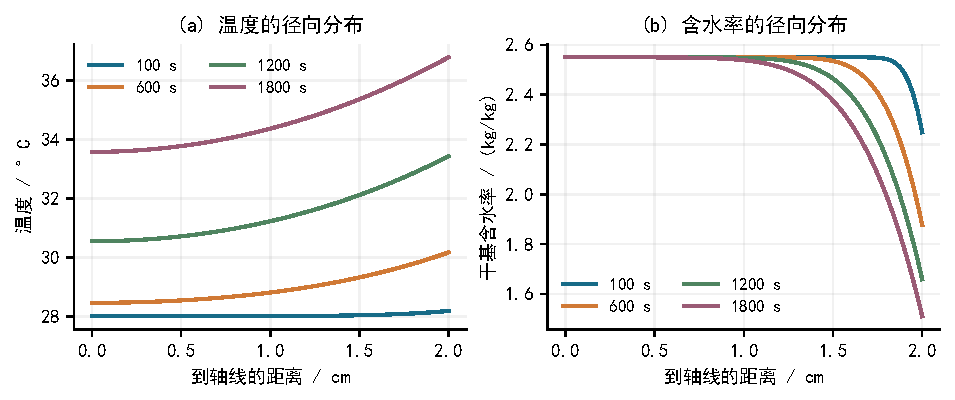
\includegraphics[width=\textwidth]{figures/q1_fields.pdf}
\caption{问题一的径向温度与含水率剖面。温度采用常数热物性，水分采用随含水率变化的扩散系数。}\label{fig:q1-fields}
\end{figure}

用初始物性作尺度估计，热扩散率为$\alpha_1=k/(\rho c_p)\approx1.69\times10^{-7}$ m$^2$/s，而初始水分扩散系数约为$4.94\times10^{-9}$ m$^2$/s。二者相差一个数量级以上。在1800 s内，$\sqrt{\alpha_1t}$约为1.74 cm，$\sqrt{D_1(C_0)t}$约为0.30 cm；后者还是未考虑近表面失水导致$D$下降的初始尺度。这个估计解释了热影响已传播至中心、水分变化仍集中于表层的趋势，但不替代非线性剖面的定量计算。

初始热Biot数为$h_TR_0/k\approx1.39$，不足以支持把圆柱温度近似为处处相同的集中参数模型。表\ref{tab:required-1}中的中心和表面差异与这一判断一致。完整结果以1 s间隔输出，径向间隔0.1 cm，分别写入\texttt{result1.xlsx}的“温度”和“水分浓度”工作表；其输出采样不同于内部0.5 s积分步长。

\section{问题二：经验物性下的全程耦合模型}
\subsection{模型实施与前3小时结果}
问题二保持固定几何与初边值条件，全部物性改用式\eqref{eq:prop23}。温度影响水分扩散，水分反过来改变有效容量和导热系数；通过每一步内的Picard迭代共同求解两个场。按照题目“统一采用附录3”的要求，0至0.5 h也使用这套经验式，而不是拼接问题一的轨迹。因此，同为1800 s，问题二与问题一得到不同的温度和表面含水率，是模型输入不同所致。

表\ref{tab:required-3}和表\ref{tab:required-4}给出0.5 h间隔的结果。0.5 h时中心温度32.1904 $^\circ$C、表面温度35.4137 $^\circ$C；3 h时中心升至49.8494 $^\circ$C、表面49.9666 $^\circ$C，径向温差已降至约0.1172 $^\circ$C。与此相比，3 h时中心含水率仍为1.7662，表面为1.0081，均明显高于0.15的要求。这说明温度接近空气平台只表明热响应接近稳定，并不等同于完成干燥。

\begin{table}[htbp]
\caption{3小时内药材的温度（单位：$^\circ$C）}\label{tab:required-3}
\centering
\small
\begin{tabular}{rrrrrr}
\toprule
时间 / h & 0 cm & 0.5 cm & 1 cm & 1.5 cm & 2 cm \\
\midrule
0.5 & 32.1904 & 32.3832 & 32.9667 & 33.9614 & 35.4137 \\
1 & 40.3822 & 40.5542 & 41.0609 & 41.8784 & 43.0001 \\
1.5 & 45.8468 & 45.9348 & 46.1930 & 46.6052 & 47.1396 \\
2 & 48.4501 & 48.4879 & 48.5983 & 48.7734 & 49.0032 \\
2.5 & 49.4669 & 49.4791 & 49.5135 & 49.5645 & 49.6617 \\
3 & 49.8494 & 49.8553 & 49.8746 & 49.9101 & 49.9666 \\
\bottomrule
\end{tabular}
\end{table}

\input{tables/table4.tex}

图\ref{fig:q2-fields}展示了这一差异：温度曲线在升温过程中整体上移并逐渐变平，含水率剖面虽整体下降，仍保持中心较高、表面较低的空间分布。完整数据按1 s和0.1 cm输出到\texttt{result2.xlsx}，温度和含水率分别存入对应工作表。

\begin{figure}[htbp]
\centering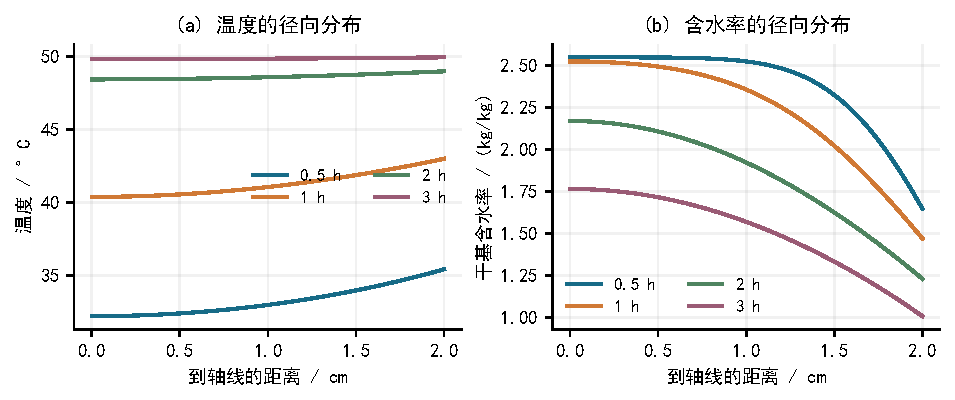
\includegraphics[width=\textwidth]{figures/q2_fields.pdf}
\caption{问题二采用附录3物性时的前3小时剖面。前半小时同样使用附录3，未与问题一的参数拼接。}\label{fig:q2-fields}
\end{figure}

\subsection{耦合的方向与后期减速机制}
由式\eqref{eq:derivatives}，升温和失水对扩散系数产生方向相反的作用。初期升温使迁移加快，同时表层含水率下降使其扩散能力变弱；随后药材接近恒温，温度提高扩散的作用基本停止，而低含水率层仍会阻碍内部水分外移。式\eqref{eq:prop23}还表明$k$、$c_p$随$C$下降而下降，因此内部温度的响应也依赖干燥进程。

这种参数耦合与加入额外水分输运热源是不同的建模选择。本文的温度场来自有效导热方程，并未在其中暗含一个未标定的蒸发冷却系数。若要利用模型进一步预测真实耗能或表面蒸发温差，还需要潜热、湿空气焓及水分相态等资料。对于本题给定的数据，本文将预测限定在上述经验温湿方程所描述的范围内。

\section{问题三：固定半径药材的达标时间}
\subsection{全域判据与事件定位}
设$C_{\mathrm{lim}}=0.15$ kg/kg。连续模型的干燥时间定义为
\begin{equation}
 t_* =\inf\{t>0:\max_{0\le r\le R_0}C(r,t)<C_{\mathrm{lim}}\}.
 \label{eq:event}
\end{equation}
对连续变化的轨迹，首次达到阈值与严格低于阈值的时间下确界相同。数值实现先检测相邻积分步的$\max_iC_i$是否跨过0.15，再在该步内用相同边界插值和后向Euler短步进行二分，选择已经满足$\max_iC_i\le0.15$的一侧作为输出。最后的全精度状态低于阈值，因此并未把仍然超标的舍入值当作达标。

采用最大值而不是平均值是题目“各处”要求的直接结果。在本文所有主轨迹中，最大值位于中心，但实现仍检查所有节点，避免把中心最湿作为未经检验的程序前提。局部温湿分布或其他边界条件改变时，最大值位置可能需要重新判断。

\subsection{达标时间与全程分布}
采用附录3物性、固定半径、0至4 h观测插值以及4 h后末点保持，得到
\begin{equation}
 \boxed{t_{*,3}=57.1726\ \mathrm h\approx57.17\ \mathrm h.}
 \label{eq:q3-answer}
\end{equation}
全精度定位时刻为205821.3125 s，最终最大含水率为0.1499999848 kg/kg。表\ref{tab:required-5}列出每6 h的含水率及末次状态。54 h时中心仍为0.1535，尽管表面已降至0.0528，仍需继续干燥约3.17 h。若根据表面先达标就停止，会误判内部状态。

\input{tables/table5.tex}

图\ref{fig:q3-drying}同时给出最大、干质量加权平均和侧表面含水率，以及代表时刻的径向剖面。平均量的定义为
\begin{equation}
 \overline C(t)=\frac{2}{R_0^2}\int_0^{R_0}C(r,t)r\,\mathrm dr
 \approx2\sum_iV_iC_i(t).\label{eq:mean-fixed}
\end{equation}
图中的平均量先于最大量跨过阈值，说明即使整体失水已较充分，中心仍可能决定最后的干燥时长。越接近终点，最大含水率曲线越平缓，少量剩余水分的迁移需要较长时间，不能用初期斜率线性外推。

\begin{figure}[htbp]
\centering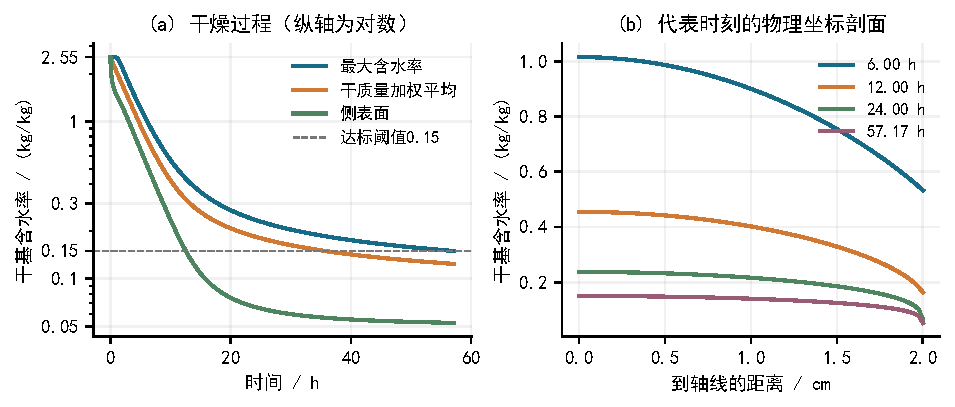
\includegraphics[width=\textwidth]{figures/q3_drying.pdf}
\caption{问题三固定半径模型的干燥过程与代表性剖面。主结果采用4 h后末点保持；图中平均值基于均匀独立干固体密度。}\label{fig:q3-drying}
\end{figure}

完整输出写入\texttt{result3.xlsx}，按60 s保存每0.1 cm位置的含水率，并额外保存实际终点。内部时间步长为0.5 s，因此不存在以60 s为单位向上取整干燥时间的问题。显示的四位小数用于满足题目制表要求，式\eqref{eq:q3-answer}保留的有效精度仍应结合后期边界假设理解。

\section{问题四：规定收缩下的材料坐标模型}
\subsection{材料运动与干固体守恒}
令$\xi$为材料标签，并规定映射
\begin{equation}
 r(\xi,t)=R(t)\xi,\qquad 0\le\xi\le1.
 \label{eq:mapping}
\end{equation}
固定轴向长度时，该映射给出径向速度$v=(\dot R/R)r$。一个材料环带的当前体积相对初始体积按$R(t)^2/R_0^2$变化。干固体守恒要求
\begin{equation}
 \frac{\partial s}{\partial t}
 +\frac1r\frac{\partial(rsv)}{\partial r}=0.
 \label{eq:dry-continuity}
\end{equation}
对空间均匀的$s(t)$，代入上述速度得$\dot s+2(\dot R/R)s=0$，从而
\begin{equation}
 s(t)=s_0\left(\frac{R_0}{R(t)}\right)^2,
 \qquad M_d=\pi Ls(t)R(t)^2=\pi Ls_0R_0^2.
 \label{eq:dry-density}
\end{equation}
这里无需指定$s_0$的具体数值即可计算干基含水率及其达标时间，因为后续质量方程的$s_0$会约去。若要报告绝对排水质量，才需要独立测量初始干固体质量，而不能从有效热学密度擅自推算。

干燥收缩可能伴随孔隙、局部密度和结构变化，已有收缩模型的综述也将不同材料和机制下的体积变化关系加以区分\cite{mayor2004}。附件2只提供外形半径轨迹，并不足以识别完整的局部力学与孔隙演化模型。本文据此采用规定形变的工程近似，而不把均匀径向收缩表述为唯一可能的微观机制。

\subsection{从真实水质量到干基含水率方程}
单位当前体积内的水质量为$sC$。水相对于固体的扩散质量通量取为$j=-sD\,C_r$。由局部水质量收支得
\begin{equation}
 \frac{\partial(sC)}{\partial t}
 +\frac1r\frac{\partial}{\partial r}\bigl[r(sCv+j)\bigr]=0.
 \label{eq:water-continuity}
\end{equation}
将式\eqref{eq:dry-continuity}乘以$C$，再从展开后的式\eqref{eq:water-continuity}中消去相应项，得到
\begin{equation}
 s\left(C_t+vC_r\right)
 =\frac1r\frac{\partial}{\partial r}\left(rsD C_r\right).
 \label{eq:material-physical}
\end{equation}
在均匀形变假设下，$s$只随时间变化，因而可以从右侧空间微分中提出并约去。又由于固定$\xi$的网格点与固体一起运动，网格速度$w=v$，有
\begin{equation}
 \left.\frac{\partial C}{\partial t}\right|_\xi
 =\left.\frac{\partial C}{\partial t}\right|_r+vC_r.
 \label{eq:chain-material}
\end{equation}
于是问题四的含水率控制方程为
\begin{equation}
 \boxed{\left.\frac{\partial C}{\partial t}\right|_\xi
 =\frac1{R(t)^2\xi}\frac{\partial}{\partial\xi}
   \left(\xi D(C,\Theta)\frac{\partial C}{\partial\xi}\right).}
 \label{eq:material-moisture}
\end{equation}
式中没有附加的收缩对流项，其原因是材料相对网格的速度为零，而不是为了让预算通过而任意删除一项。这一推导依赖$v=w$、固定长度和均匀干密度三个条件；如果采用非均匀收缩或不同的网格运动，需要重新保留相对网格输运以及空间变化的$s$。

温度采用同一材料导数及有效体积热容，写成
\begin{equation}
 a(C)\left.\frac{\partial T}{\partial t}\right|_\xi
 =\frac1{R(t)^2\xi}\frac{\partial}{\partial\xi}
   \left(\xi k(C)\frac{\partial T}{\partial\xi}\right).
 \label{eq:material-heat}
\end{equation}
这一温度方程与水分方程在运动描述上相同，但热量闭合仍为前述有效导热近似。两式均使用附录4物性，并在$\xi=0$施加零梯度，在$\xi=1$施加
\begin{equation}
 -\frac{k}{R}T_\xi=h_T(T_s-T_{\mathrm{air}}),
 \qquad-\frac{D}{R}C_\xi=h_m(C_s-C_{\mathrm{eq}}).
 \label{eq:material-robin}
\end{equation}
侧面真实水质量通量为$s h_m(C_s-C_{\mathrm{eq}})$。乘以侧面积$2\pi RL$后，与总体水质量的变化一致。因此$s$虽从局部含水率方程中约去，在真实质量解释中仍不可省略。

定义材料参考积分$I(t)=\int_0^1C(\xi,t)\xi\,\mathrm d\xi$，由式\eqref{eq:material-moisture}及边界条件有
\begin{equation}
 \frac{\mathrm dI}{\mathrm dt}=-\frac{h_m}{R(t)}(C_s-C_{\mathrm{eq}}),
 \qquad \frac{M_w}{M_d}=2I(t).
 \label{eq:material-budget}
\end{equation}
式\eqref{eq:material-budget}给出了一个直接可计算的质量预算，并与式\eqref{eq:discrete-budget}对应。表格与图中的平均含水率始终采用这一分母，不使用单纯的几何积分$R(t)^2I(t)$代替干基水质量。

\subsection{有效密度与质量定义的一致性}\label{sec:density}
如果将附录4的$\rho(C)=760+90C$同时解释为真实的局部湿药材总体密度，那么干基定义会强制给出$s_\rho(C)=\rho(C)/(1+C)$。固定长度、规定半径和这一密度解释所推算的总干质量为
\begin{equation}
 M_{d,\rho}(t)=2\pi LR(t)^2
 \int_0^1\frac{760+90C(\xi,t)}{1+C(\xi,t)}\xi\,\mathrm d\xi.
 \label{eq:rho-counterexample}
\end{equation}
将本文主轨迹代入式\eqref{eq:rho-counterexample}，所得到的$M_{d,\rho}/M_{d,\rho}(0)$在保存的时间点上最低为0.7196，发生于约7.22 h，终点为0.8903，见图\ref{fig:q4-mass}。这意味着该额外解释并不满足干固体质量恒定，偏差也远大于离散预算的舍入误差。

\begin{figure}[htbp]
\centering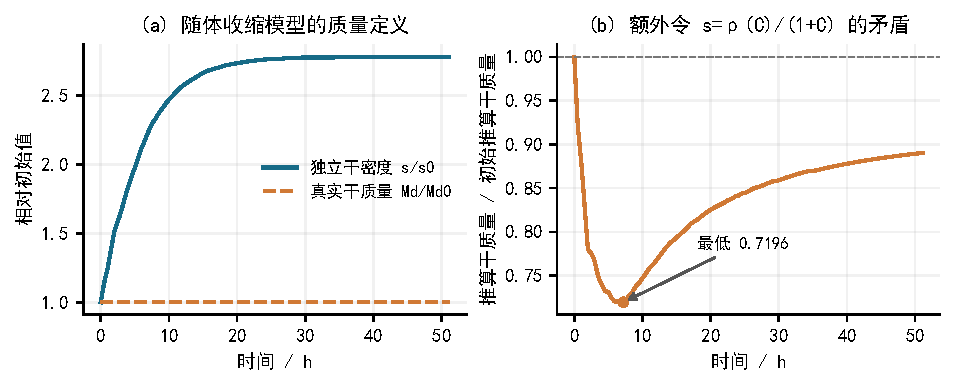
\includegraphics[width=\textwidth]{figures/q4_mass_definition.pdf}
\caption{问题四的两种密度解释。左图为独立干密度保证的质量守恒；右图检验额外把热学密度等同于真实湿密度时的推算干质量。}\label{fig:q4-mass}
\end{figure}

因此本文保留题目的经验物性数值，但限定其热学用途，以式\eqref{eq:dry-density}独立描述守恒干固体。这样得到的是条件清楚、内部一致的有效模型。它没有证明题目的密度公式在真实材料中的含义只能如此解释；若要求$\rho$同时具有严格的湿料质量意义，则必须补充并修改形变、轴向长度或多相结构关系，不能继续保持当前所有假设不变。

\subsection{主结果与收缩域上的输出}
用均值平台求解式\eqref{eq:material-moisture}至式\eqref{eq:material-robin}，得到
\begin{equation}
 \boxed{t_{*,4}=51.0913\ \mathrm h\approx51.09\ \mathrm h.}
 \label{eq:q4-answer}
\end{equation}
全精度终点为183928.625 s，最大含水率0.1499999894 kg/kg，半径为1.2000 cm，侧表面含水率按四位小数显示为0.0526。表\ref{tab:required-6}给出每6 h的实际位置输出及终点。6 h时半径已为1.3740 cm，故1.5 cm、2 cm处已经不在药材内，相应位置用横线表示；Excel中保留为空值，不能填零或把表面值外延到不存在的材料区域。

\begin{table}[htbp]
\caption{随体收缩药材烘干过程的干基含水率（单位：kg/kg）}\label{tab:required-6}
\centering
\footnotesize
\begin{tabular}{rrrrrrrr}
\toprule
时间 / h & 0 cm & 0.5 cm & 1 cm & 1.5 cm & 2 cm & 侧表面 & 半径 / cm \\
\midrule
6 & 1.7188 & 1.5370 & 1.0221 & --- & --- & 0.4205 & 1.3740 \\
12 & 0.7374 & 0.6544 & 0.4082 & --- & --- & 0.1669 & 1.2480 \\
18 & 0.4087 & 0.3686 & 0.2397 & --- & --- & 0.0892 & 1.2140 \\
24 & 0.2851 & 0.2610 & 0.1790 & --- & --- & 0.0673 & 1.2040 \\
30 & 0.2263 & 0.2094 & 0.1492 & --- & --- & 0.0595 & 1.2010 \\
36 & 0.1928 & 0.1796 & 0.1316 & --- & --- & 0.0559 & 1.2000 \\
42 & 0.1712 & 0.1604 & 0.1200 & --- & --- & 0.0541 & 1.2000 \\
48 & 0.1561 & 0.1468 & 0.1116 & --- & --- & 0.0530 & 1.2000 \\
51.0913 & 0.1500 & 0.1413 & 0.1081 & --- & --- & 0.0526 & 1.2000 \\
\bottomrule
\end{tabular}
\end{table}


输出表中$r=0.5$ cm等列对应固定的物理空间距离，不是固定材料标签。对每个输出时刻，先计算当前半径，再以$\xi=r/R(t)$从材料网格插值；若$r>R(t)$则不输出材料数值。侧表面单列直接取$\xi=1$，因此即使半径不恰好落在0.1 cm的采样网格上，也能保留准确的表面状态。\texttt{result4.xlsx}按60 s输出并额外保留终点，避免收缩后表格位置含义不清。

图\ref{fig:q4-drying}展示主模型的全程下降与代表性剖面。后期曲线仍存在明显尾段，中心是达标约束的控制位置。终点平均含水率约为0.11835，低于中心的阈值0.15，说明达标时内部并非处处具有相同含水率。只要所有位置低于上限，保留这种空间差异并不违反题目要求。

\begin{figure}[htbp]
\centering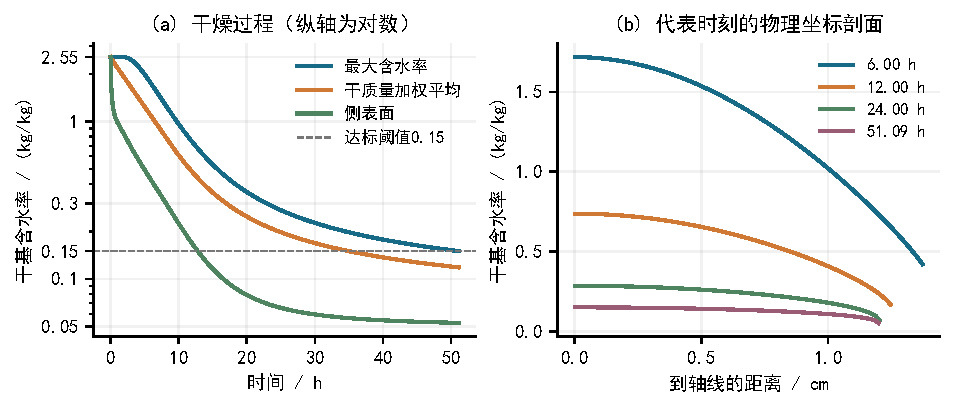
\includegraphics[width=\textwidth]{figures/q4_drying.pdf}
\caption{问题四材料坐标、末小时均值平台下的干燥结果。右图横轴为当前物理距离，各条曲线的终点随半径改变。}\label{fig:q4-drying}
\end{figure}

\section{模型对照、数值验证与敏感性分析}
\subsection{同物性、同边界的严格对照}\label{sec:ablation}
为了单独考察几何和运动描述，三组对照均使用附录4物性、均值平台、81节点、0.5 s步长及相同初始状态。第一组固定$R=R_0$，第二组采用本文随体收缩，第三组将移动边界应用在没有固体径向运动的Eulerian扩散场上。这第三组属于不同的运动假设，保留它是为了说明坐标变换和材料守恒的区别，不将其视为本文主解。

对于没有物质速度的Eulerian扩散方程，单纯变换$r=R(t)\xi$会出现
\begin{equation}
 \left.C_t\right|_\xi
 =\frac1{R^2\xi}\partial_\xi(\xi D C_\xi)
  +\frac{\dot R}{R}\xi C_\xi.
 \label{eq:eulerian-comparison}
\end{equation}
链式法则中的符号本身没有错误，但它与式\eqref{eq:material-moisture}描述的物理运动不同。此时几何积分的预算包含$R\dot R C_s$，即边界扫掠项：
\begin{equation}
 \frac{\mathrm d}{\mathrm dt}(R^2I)
 =-Rh_m(C_s-C_{\mathrm{eq}})+R\dot R C_s.
 \label{eq:swept-budget}
\end{equation}
所以通过几何积分预算，并不能证明以守恒干固体为分母的水质量正确。把“离散守恒”与“守恒的物理量是什么”同时写清，才能判断两种运动描述的适用性。

表\ref{tab:ablation}与图\ref{fig:q4-ablation}给出完整对照。相同物性和平台下，固定半径需要129.8561 h，随体收缩需要51.0913 h，缩短78.7649 h，约为60.66\%；Eulerian移动对照为52.6548 h，比材料坐标结果增加1.5636 h。可见，固定半径与移动域的巨大差异主要出现在几何路径改变后，而额外扫掠输运只解释两种移动描述之间的一部分差别。

\begin{table}[htbp]
\centering\caption{问题四同物性、同均值平台的运动与几何对照}\label{tab:ablation}
\begin{tabular}{lrrr}\toprule
计算情景 & 初始半径/cm & 终点半径/cm & 达标时间/h\\\midrule
固定半径 & 2.0000 & 2.0000 & 129.8561\\
随体归一化坐标 & 2.0000 & 1.2000 & 51.0913\\
Eulerian移动边界对照 & 2.0000 & 1.2000 & 52.6548\\\bottomrule
\end{tabular}
\end{table}

收缩使水分迁移距离缩短，同时提高单位干质量对应的侧面交换作用。半径由0.02 m降至0.012 m后，在归一化方程中$1/R^2$增加为初始的约2.778倍，$h_m/R$增加为约1.667倍。这一尺度变化可以解释缩短方向，但物性随温湿场变化，且半径并非瞬间缩至终值，故不能直接用$0.6^2$乘固定半径时长作为精确答案。

\subsection{边界延续情景对结果的影响}
材料坐标下，末点保持得到50.8235 h，末小时均值平台得到51.0913 h，名义平台得到51.0899 h。末小时均值与名义平台仅相差约5.13 s，而末点保持比均值平台提前约16.07 min，结果见图\ref{fig:q4-ablation}左图。由于末点的温度略高、水分变量略低，其延续条件更有利于干燥，时间缩短的方向与方程一致。

\begin{figure}[htbp]
\centering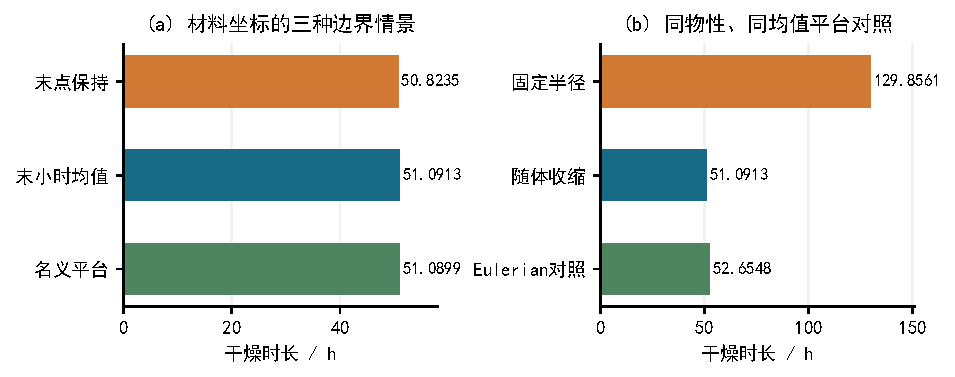
\includegraphics[width=\textwidth]{figures/q4_scenarios_ablation.pdf}
\caption{问题四的边界情景与严格对照。左图均为材料坐标；右图统一采用附录4物性和末小时均值平台。}\label{fig:q4-ablation}
\end{figure}

三种相邻平台情景得到约50.82至51.09 h的范围，只是指定的边界延续比较，不是统计置信区间，也不覆盖未给出的全部工艺可能。若实际后期升温、降温、间歇通风或水分平台改变，结果需要重新计算。本文选择均值平台的依据是利用后段多个观测值形成代表性稳定水平，而不是已知未来边界必然恒定。

问题三和问题四的主时长分别为57.17 h和51.09 h，虽然数值相近，不能据此说收缩仅带来约6 h的收益。两问使用的扩散系数前因子及含水率指数不同，热物性也不同，边界延续还存在差别。表\ref{tab:ablation}的配对比较才是在指定附录4物性下讨论收缩影响的依据。不同对照所回答的问题不同，合并解释会掩盖参数变化与运动学变化的各自作用。

\subsection{求解器与守恒验证}\label{sec:validation}
先以可独立构造的问题检查离散实现，再考察非线性主模型的收敛。Thomas算法与独立带状矩阵求解比较，最大差约为$1.07\times10^{-14}$。对移动几何下的常数场，分别检查收缩和膨胀、Euler和BDF2组合，最大误差约为$4.34\times10^{-10}$，用于检验几何离散的一致性。该常数场试验检验的是离散几何恒等式，不能替代第\ref{sec:density}节的物理质量解释。

圆柱径向离散的独立验证采用Robin特征模态。在常系数、零外界扰动的情况下，取
\begin{equation}
 u(r,t)=J_0(\lambda r/R_0)
 \exp(-\alpha\lambda^2t/R_0^2),\quad
 \lambda J_1(\lambda)=\mathrm{Bi}_T J_0(\lambda),
 \label{eq:eigenmode}
\end{equation}
其中$J_0,J_1$为第一类Bessel函数。使用解析初值，时间步长0.05 s，积分到100 s，与解析场比较。表\ref{tab:solver-validation}列出结果：节点由21增至41、81时，最大场误差持续下降，支持轴线、径向控制体和Robin表面项的正确离散。

\begin{table}[htbp]
\centering\caption{独立数值验证结果}\label{tab:solver-validation}
\begin{tabular}{lr}\toprule
验证对象与误差定义 & 误差\\\midrule
Thomas与独立带状求解器：最大绝对差 & $1.0658\times10^{-14}$\\
移动几何常数场：最大绝对差 & $4.3396\times10^{-10}$\\
Robin模态，21节点：最大绝对场误差 & $9.1433\times10^{-5}$\\
Robin模态，41节点：最大绝对场误差 & $2.2193\times10^{-5}$\\
Robin模态，81节点：最大绝对场误差 & $4.8579\times10^{-6}$\\
8点界面求积与自适应积分：最大相对差 & $3.6731\times10^{-9}$\\
材料坐标Euler独立算例：累计相对水分残差 & $3.0477\times10^{-15}$\\
材料坐标BDF2独立算例：累计相对水分残差 & $1.4368\times10^{-14}$\\\bottomrule
\end{tabular}
\end{table}

非线性界面求积的验证沿三个不同含水率区间和45至50 $^\circ$C的重构温度路径进行，分别用自适应数值积分和8点Gauss规则计算式\eqref{eq:edge-integral}，最大相对差为$3.67\times10^{-9}$。它针对的是界面系数积分，而不是对整个药材模型的外部实验拟合。

问题四主轨迹的材料参考积分累计相对残差约为$4.67\times10^{-14}$，与离散预算一致。该主轨迹统计覆盖内部整步，不包含最后事件二分产生的短步；二维端面对照另有包含末次短步的完整预算。报告统计范围，可以避免将一个未纳入累计量的子步骤误称为已经验证。所有这些残差均衡量代数实现和数值收支，不表示物理预测误差已经达到机器精度。

\subsection{时间、空间和插值收敛}\label{sec:convergence}
对问题四主模型，所有收敛算例统一使用材料坐标和均值平台。空间试验固定$\Delta t=1$ s，分别采用41、81、161节点；时间试验固定81节点，使用4、2、1、0.5 s；另计算BDF2和线性边界插值的情景。表\ref{tab:convergence}和图\ref{fig:q4-convergence}给出实际达标时间。

\begin{table}[htbp]
\centering\caption{问题四当前材料模型的离散与插值比较}\label{tab:convergence}
\begin{tabular}{lrrlr}\toprule
比较项 & 节点数 & 步长/s & 方法与插值 & 达标时间/h\\\midrule
空间粗级 & 41 & 1 & Euler，PCHIP & 51.0988021\\
空间中级 & 81 & 1 & Euler，PCHIP & 51.0916146\\
空间细级 & 161 & 1 & Euler，PCHIP & 51.0897917\\
时间粗级 & 81 & 4 & Euler，PCHIP & 51.0935938\\
时间中级 & 81 & 2 & Euler，PCHIP & 51.0922743\\
主结果 & 81 & 0.5 & Euler，PCHIP & 51.0912847\\
时间格式 & 81 & 1 & BDF2，PCHIP & 51.0909549\\
边界插值 & 81 & 1 & Euler，线性 & 51.0916146\\\bottomrule
\end{tabular}
\end{table}

固定1 s时，81节点加密到161节点，时间改变0.0018229 h，即6.5625 s；固定81节点时，1 s减至0.5 s，时间改变1.1875 s。Euler与BDF2在1 s下相差2.3750 s。线性插值与PCHIP在该次试验中给出相同的事件输出，说明在当前时刻定位分辨率下没有分辨出两者对达标时间的差异；这并不表示任意时刻的完整温湿场都严格相同。

\begin{figure}[htbp]
\centering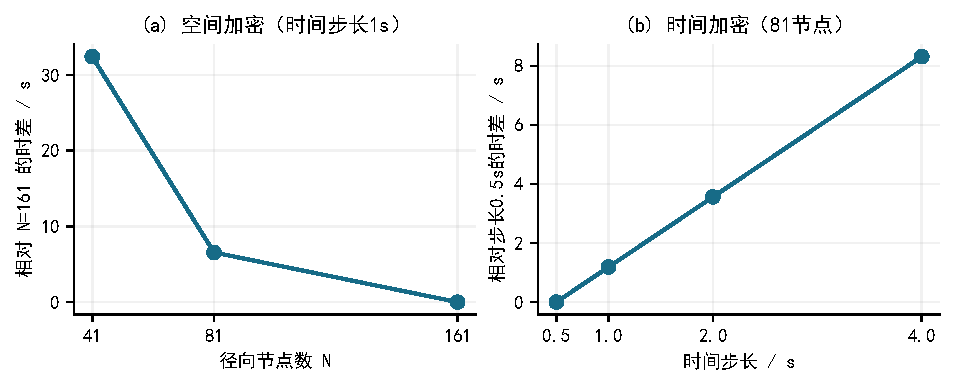
\includegraphics[width=\textwidth]{figures/q4_convergence.pdf}
\caption{问题四材料模型的空间与时间加密。纵轴分别相对于最细空间和最细时间算例，不能作为连续解误差的严格上界。}\label{fig:q4-convergence}
\end{figure}

这些结果支持51.09 h不是明显的离散偶然值。主轨迹的最终事件括区宽度为0.0625 s，但这一宽度只描述给定离散轨迹上的定位分辨率，不能作为总预测精度。特别是，均值与末点边界导致的约16 min差异远大于此次加密带来的秒级变化，因此继续显著缩小时间步长，并不能消除后期工艺边界的信息缺口。

\subsection{参数敏感性}
为考察经验参数的不确定影响，分别给$D,h_m,h_T,k$乘以0.8、0.9、1.0、1.1和1.2，其余条件保持不变。每次重新求解完整非线性轨迹，统一使用81节点、1 s、材料坐标和均值平台。基准时长为51.0916146 h，稍异于0.5 s的主结果，故所有百分比均相对于本节共同基准计算。$D$的倍率作用于整个经验函数，不改变其对$C,\Theta$的函数形式；参数变化时半径轨迹仍按附件2规定。

表\ref{tab:sensitivity}和图\ref{fig:q4-sensitivity}显示，扩散系数对时长的影响最大。$D$减小20\%时，达标时间增至62.3506 h，增加22.04\%；$D$增大20\%时降至43.6211 h，减少14.62\%。响应并非对称的线性关系，这与扩散系数随状态变化及达标阈值位于后期减速段有关。

\begin{table}[htbp]
\centering\caption{问题四单参数倍率试验的达标时间（单位：h）}\label{tab:sensitivity}
\begin{tabular}{lrrrrr}\toprule
参数 & $\times0.8$ & $\times0.9$ & $\times1.0$ & $\times1.1$ & $\times1.2$\\\midrule
$D$ & 62.3506 & 56.0918 & 51.0916 & 47.0116 & 43.6211\\
$h_m$ & 51.7773 & 51.3827 & 51.0916 & 50.8708 & 50.6994\\
$h_T$ & 51.1098 & 51.0997 & 51.0916 & 51.0851 & 51.0797\\
$k$ & 51.0960 & 51.0936 & 51.0916 & 51.0901 & 51.0888\\\bottomrule
\end{tabular}
\end{table}

\begin{figure}[htbp]
\centering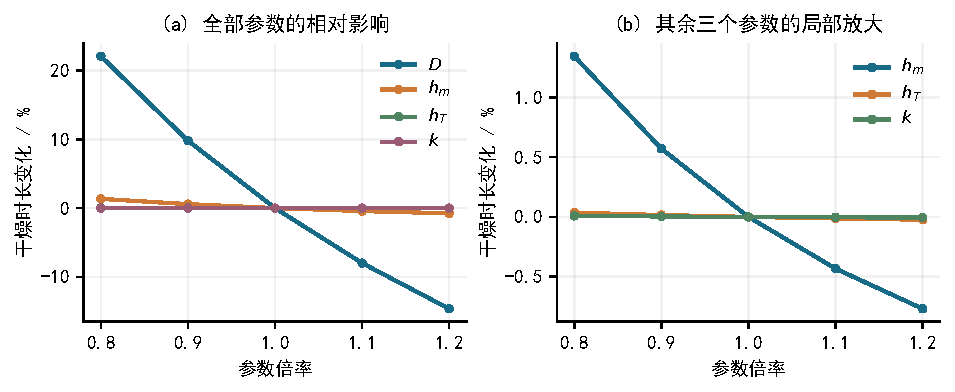
\includegraphics[width=\textwidth]{figures/q4_sensitivity.pdf}
\caption{问题四参数倍率对达标时间的影响。右图将其余参数的响应单独放大；两图百分比采用同一1 s基准轨迹。}\label{fig:q4-sensitivity}
\end{figure}

对$h_m$，减小20\%延长约1.34\%，增大20\%缩短约0.77\%，明显弱于同幅度的$D$变化。$h_T$和$k$的20\%变化对全程时长的影响更小，最大相对变化分别约0.0355\%与0.0087\%。这与药材在初期已接近热平台、后期主要受低含水率扩散制约的结果相符。这里的结论针对达标时间，不等于热参数对早期温度场也同样不敏感。

指定倍率试验没有给参数建立概率分布，因此表\ref{tab:sensitivity}不产生置信区间。由于缺少真实参数分布及4 h后工艺记录，本文不将大量随机抽样的分位数包装成经过数据支持的预测概率。若进一步开展不确定性量化，应先确定扩散系数和边界延续的可用信息，再决定抽样规模，而不能以增加计算量代替物理输入。

\section{轴对称端面对照与适用范围}\label{sec:endface}
\subsection{二维模型与配对设计}
为检验一维近似，对问题四主模型增加轴向坐标$z$，利用中截面对称只计算$0\le z\le H=0.125$ m。在相同随体径向形变下，水分方程为
\begin{equation}
 C_t=\frac1{R(t)^2\xi}\partial_\xi(\xi D C_\xi)
       +\partial_z(D C_z),\label{eq:2d}
\end{equation}
温度方程采用同样的空间算子，以$a$乘时间导数、以$k$替换$D$。在$z=0$施加对称条件；在$z=H$施加与侧面相同的$h_T,h_m$和$C_{\mathrm{eq}}$。端面系数相同是一项用于对照的暴露条件，题目并未独立测定端面的传递系数。

径向采用与一维相同的控制体，轴向节点使用$z=H[1-(1-u)^2]$，其中$u$均匀取点，以增加端面附近的分辨率。时间上使用全隐式Euler与Picard迭代，线性子问题采用稀疏直接求解。关闭端面交换时，二维场应退化为沿轴向重复的一维解；开放端面后，再与相同径向网格和时间步长的一维解配对，避免将离散设置变化当成端面作用。

令轴向控制体宽度为$W_j$，参考半域体积权重为$V_{\mathrm{ref}}=\sum_{ij}V_iW_j=H/2$，则
\begin{equation}
 \begin{aligned}
 \overline C&=\frac{\sum_{ij}V_iW_jC_{ij}}{V_{\mathrm{ref}}},\\
 F_s&=\frac{h_m}{RV_{\mathrm{ref}}}\sum_jW_j(C_{s,j}-C_{\mathrm{eq}}),\qquad
 F_e=\frac{h_m}{V_{\mathrm{ref}}}\sum_iV_i(C_{i,H}-C_{\mathrm{eq}}).
 \end{aligned}
 \label{eq:2d-budget}
\end{equation}
其中$F_s,F_e$分别为相对于总干质量的侧面和端面失水速率。完整圆柱的周向系数、两个端面和对称半域倍数已在分子分母中约去，故不会因为只计算一半长度而漏掉一个端面。二维预算逐步检查$\overline C^n-\overline C^{n-1}+\Delta t(F_s+F_e)=0$，并包含最后事件短步。

\subsection{结果与解释}
表\ref{tab:endface-paired}列出闭端退化试验及两级开放端面对照。闭端计算的二维场与重复的一维场在代表时刻的最大温差约为$1.95\times10^{-12}$ K，最大含水率差约为$4.49\times10^{-14}$ kg/kg，说明该实现能够回到一维模型。

\begin{table}[htbp]
\centering\caption{端面试验与同设置一维解的配对结果}\label{tab:endface-paired}
\begin{tabular}{lrrrr}\toprule
端面设置 & 径向$\times$轴向节点 & 步长/s & 一维时间/h & 二维时间/h\\\midrule
关闭交换 & $41\times9$ & 30 & 51.1178874 & 51.1178874\\
开放粗级 & $41\times25$ & 30 & 51.1178874 & 51.1178874\\
开放细级 & $81\times37$ & 15 & 51.1008301 & 51.1008301\\\bottomrule
\end{tabular}
\end{table}

两级开放计算在当前事件定位分辨率内都没有分辨出配对达标时差。细级二维全程相对水分预算残差约为$5.61\times10^{-14}$，累计端面排水占全部排水的3.9032\%。细级配对时间51.1008301 h比0.5 s主结果略大，是较粗时间设置下的数值结果；不能把这一绝对差直接当作端面误差。

另一方面，二维开放端面确实改变了平均含水率。表\ref{tab:endface-mean}与图\ref{fig:q4-endface}显示，4 h时一维平均值为1.42299055，二维降至1.37869807，变化约$-3.1126\%$；终点一维为0.11834815，二维为0.11607800，变化约$-1.9182\%$。因此，“未分辨出全域最大值达标时差”与“平均量和端部场有变化”可以同时成立。

\begin{table}[htbp]
\centering\caption{细级端面对照在相同时刻的平均含水率}\label{tab:endface-mean}
\begin{tabular}{rrrr}\toprule
时间/h & 一维平均$C$ & 二维平均$C$ & 相对变化/\%\\\midrule
0.5000 & 2.34383354 & 2.32874268 & $-0.6439$\\
4.0000 & 1.42299055 & 1.37869807 & $-3.1126$\\
24.0000 & 0.20541408 & 0.19931230 & $-2.9705$\\
51.1008 & 0.11834815 & 0.11607800 & $-1.9182$\\\bottomrule
\end{tabular}
\end{table}

\begin{figure}[htbp]
\centering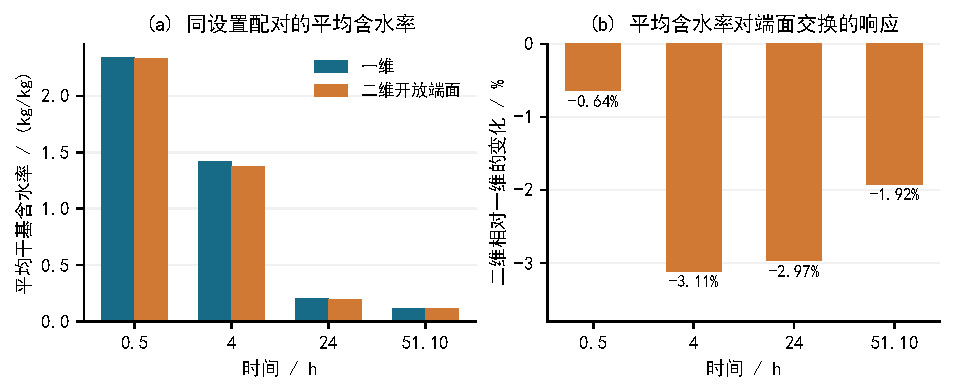
\includegraphics[width=\textwidth]{figures/endface.pdf}
\caption{同网格、同时间步长下，端面交换对平均含水率的影响。此处比较量为平均含水率，而不是全域最大含水率的达标时间。}\label{fig:q4-endface}
\end{figure}

中截面到端面的距离0.125 m大于径向扩散距离0.02至0.012 m，端部失水可先改变端部附近的局部场，而控制最迟达标的中心区域仍主要通过径向排水。这一尺度解释与本组对照相符，但本文不把重合的离散事件括区解释为连续偏微分方程的严格误差上界。不同端面传递系数、不同长径比或存在轴向收缩时，需要重新检验。

\section{模型评价与结论}
\subsection{有效性与局限}
本文以相同控制体结构求解四问，使几何、物性和边界的改变可以分开追踪。圆柱权重避免了中心奇点，隐式非线性迭代能够处理长达数十小时的低含水率尾段；解析模态、独立线性求解、界面求积和时间空间加密分别检验不同数值环节。问题四从干固体连续方程出发定义水质量，明确了材料坐标中无相对网格输运的条件，并以同物性对照解释固定与收缩半径的时间差。

模型的限制主要来自可用物理信息。第一，4 h后边界延续是情景，尚无后续工艺观测。第二，空气变量到等效表面含水率的映射缺少吸附数据，传质边界属于经验闭合。第三，半径仅由附件规定，均匀径向形变和热学有效密度解释需要独立实验支持；参数扫描中也没有重新求解含水率影响收缩的力学反馈。第四，温度方程未描述潜热、多相焓和结构损伤，不能用于直接推断能耗或品质变化。第五，端面对照只验证了特定暴露条件，不能推广为所有局部场的端面作用均可忽略。

上述不确定性对不同输出量的影响并不相同。端面对最大值达标时间和平均含水率的不同作用已经说明，不能把所有误差来源排成一条适用于任何指标的固定大小顺序。对于本题的时长预测，当前网格与时间步比较已经达到秒级差异；对于平均失水量、端部状态或能耗，则需要针对相应物理量补充数据和验证。

\subsection{四问结论}
问题一得到表\ref{tab:required-1}、表\ref{tab:required-2}及图\ref{fig:q1-fields}所示结果。前30 min热量向中心传播明显快于水分变化：1800 s时中心与表面温度分别为33.5764 $^\circ$C和36.7861 $^\circ$C，表面含水率降至1.5104，中心仍接近2.55。问题二在全程使用附录3后，3 h时中心温度升至49.8494 $^\circ$C，但最大含水率仍为1.7662，说明达到近恒温状态远早于完成干燥。

问题三在固定半径、附录3物性和末点延续条件下，首次全域达标时间为57.1726 h，完整水分剖面见表\ref{tab:required-5}。问题四在规定半径、均匀随体径向收缩、独立干固体守恒、经验有效热物性及末小时均值平台下，推荐时间为51.0913 h，结果见表\ref{tab:required-6}和图\ref{fig:q4-drying}。末点保持与名义平台分别得到50.8235 h和51.0899 h，作为并列边界情景保留。

严格配对计算表明，同附录4物性和均值平台下，固定半径需要129.8561 h，收缩显著缩短迁移距离，材料坐标解为51.0913 h。Eulerian扫掠边界对照为52.6548 h，其守恒对象与材料水质量不同，不能替代主模型。参数试验中扩散系数对时长最敏感；端面对照支持在本文条件下用径向模型预测最迟达标时刻，同时提示平均含水率仍受端面交换影响。以上结论连同四份Excel，构成给定资料与明确假设下的完整计算回答。

\clearpage
\CumcmAIUsed{模型推导讨论、物理假设审查、数值程序编写与调试、结果核对、文献检索和论文初稿撰写}

\bibliographystyle{gbt7714-numerical}
\bibliography{references}

\clearpage
\appendix
\titleformat{\section}{\centering\heiti\zihao{3}\bfseries}{附录~\thesection}{0.8em}{}
\section{支撑材料及运行说明}\label{app:materials}
表\ref{tab:support-files}列出与本文结果对应的文件。程序按模块组织，所有计算使用相对路径读取同一目录内的数据；原始Excel可与转换后的CSV逐项核对。以下程序清单给出正文涉及的求解、验证、对照和导出代码。源码中的模型编号1、2、4分别表示问题一、问题二和三、问题四；编号差异没有物理量纲含义。

\begin{longtable}{p{0.48\textwidth}p{0.43\textwidth}}
\caption{支撑材料文件列表}\label{tab:support-files}\\
\toprule 文件或目录 & 内容与用途\\\midrule\endfirsthead
\toprule 文件或目录 & 内容与用途\\\midrule\endhead
\bottomrule\endfoot
\texttt{result1.xlsx}、\texttt{result2.xlsx} & 温度和水分浓度，1 s时间间隔、0.1 cm空间间隔\\
\texttt{result3.xlsx}、\texttt{result4.xlsx} & 水分浓度，60 s时间间隔并包含终点；问题四保留独立表面列\\
\texttt{data/boundary.csv}、\texttt{data/radius.csv} & 附件1与附件2的数值转存，保持原始时刻与单位\\
\texttt{run.py}、\texttt{physics/}、\texttt{solver/} & 四问主计算、物性、外部边界和一维有限体积求解器\\
\texttt{experiments/} & 问题四三种平台、几何运动对照、收敛与单参数扫描\\
\texttt{validation/}、\texttt{tests/} & 二维端面对照、输出一致性检查及独立数值测试\\
\texttt{export/} & 从全精度结果形成题目指定工作表\\
\texttt{results/q1.npz}至\texttt{q4.npz} & 按规定输出频率保存的全精度径向轨迹\\
\texttt{results/q1.json}至\texttt{q4.json} & 物性选择、网格步长、边界和达标状态\\
\texttt{results/}中的比较CSV与JSON & 本文收敛、参数与端面比较的数值记录\\
\texttt{paper/prepare\_paper\_assets.py} & 从现有数值轨迹生成本文图与六张题目结果表\\
\texttt{AI工具使用详情.pdf} & 已知AI参与环节、提示方式及核验情况说明\\
\end{longtable}

主计算依赖Python、NumPy、SciPy和Numba；绘图依赖Matplotlib；现有Excel导出程序依赖Node.js及\texttt{@oai/artifact-tool}。本文数值结果使用Python 3.10、NumPy 1.26.4、SciPy 1.15.2及Numba 0.67.0生成。二维计算比一维更耗时，但只需执行本文给出的三个配对算例，不要求多卡设备。

在程序根目录执行\texttt{python run.py}可依次计算四问；执行实验目录中的问题四对照与参数脚本可生成本文相应表格。二维脚本的三个设置依次为径向41、轴向9、30 s且关闭端面；径向41、轴向25、30 s且开放端面；径向81、轴向37、15 s且开放端面，均启用同设置一维配对。主结果的半径列以m存储，Excel输出时转换为cm；时间轨迹统一用s存储，正文表格按题目要求转换为h。

\section{完整源程序}
\lstset{basicstyle=\ttfamily\scriptsize,basewidth=0.5em,lineskip=0pt}
\Needspace{9\baselineskip}
\subsection{主计算入口}
文件：\path{run.py}。
\lstinputlisting[language=Python,caption={主计算入口}]{code/run.py}
\Needspace{9\baselineskip}
\subsection{经验物性与界面扩散系数}
文件：\path{physics/material.py}。
\lstinputlisting[language=Python,caption={经验物性与界面扩散系数}]{code/physics/material.py}
\Needspace{9\baselineskip}
\subsection{观测插值和边界延续}
文件：\path{physics/boundary.py}。
\lstinputlisting[language=Python,caption={观测插值和边界延续}]{code/physics/boundary.py}
\Needspace{9\baselineskip}
\subsection{一维有限体积求解器}
文件：\path{solver/fvm_cpu.py}。
\lstinputlisting[language=Python,caption={一维有限体积求解器}]{code/solver/fvm_cpu.py}
\Needspace{9\baselineskip}
\subsection{问题四边界与几何对照}
文件：\path{experiments/q4_release.py}。
\lstinputlisting[language=Python,caption={问题四边界与几何对照}]{code/experiments/q4_release.py}
\Needspace{9\baselineskip}
\subsection{问题四收敛及参数试验}
文件：\path{experiments/q4_validation.py}。
\lstinputlisting[language=Python,caption={问题四收敛及参数试验}]{code/experiments/q4_validation.py}
\Needspace{9\baselineskip}
\subsection{主结果一致性检查}
文件：\path{validation/q4_contract.py}。
\lstinputlisting[language=Python,caption={主结果一致性检查}]{code/validation/q4_contract.py}
\Needspace{9\baselineskip}
\subsection{轴对称端面求解与配对比较}
文件：\path{validation/endface_benchmark.py}。
\lstinputlisting[language=Python,caption={轴对称端面求解与配对比较}]{code/validation/endface_benchmark.py}
\Needspace{9\baselineskip}
\subsection{独立数值验证}
文件：\path{tests/test_solver.py}。
\lstinputlisting[language=Python,caption={独立数值验证}]{code/tests/test_solver.py}
\Needspace{9\baselineskip}
\subsection{Excel数值准备}
文件：\path{export/prepare_outputs.py}。
\lstinputlisting[language=Python,caption={Excel数值准备}]{code/export/prepare_outputs.py}
\Needspace{9\baselineskip}
\subsection{Excel模板导出}
文件：\path{export/workbooks.mjs}。
\lstinputlisting[language=Java,caption={Excel模板导出}]{code/export/workbooks.mjs}
\Needspace{9\baselineskip}
\subsection{论文图与结果表生成}
文件：\path{paper/prepare_paper_assets.py}。
\lstinputlisting[language=Python,caption={论文图与结果表生成}]{code/paper/prepare_paper_assets.py}

